Im Folgenden sollen die beschriebenen Ergebnisse aus den vorherigen Abschnitten \ref{sec:ergebnisseSichtpruefungDurchLichtstreuung} und \ref{sec:ergebnisseDeflektometrischeRegistrierung} aufgegriffen und bewertet werden.
Das Ziel ist es abhängig vom Anwendungsfall ein passendes Verfahren vorzuschlagen und die Schwächen und Stärken der Verfahren darzulegen.

\p
Für das Verfahren \glqq Sichtprüfung durch Lichtstreuung\grqq ~fällt im Abschnitt \ref{sec:ergebnisseSichtpruefungDurchLichtstreuung} auf, dass es sich besonders gut für die Durchlichtauswertung von transparenten Prüfobjekten eignet.
Es ist möglich bereits sehr kleine Defekte, wie z. B. sehr leichte Kratzer oder Laser-Gravuren auf den Objektoberflächen zu erkennen (siehe Abbildung \ref{tikz:abbErkennbareKleineDefekteLichtstreuung}).

% Abbildung: Erkennbare kleine Defekte
{
	\begin{figure}[H]
		\centering
		\begin{tikzpicture}[every node/.style={inner sep=0,outer sep=0}]

	\node [anchor=north east] (img1) at (-0.03\textwidth,0) {\includegraphics[width=.4\textwidth]{05_ergebnisse/ergDiskussion/figures/lasergravur}};
	\node [below=0.2cm of img1] {Ausschnitt von Brillenglas 1};
	\node [anchor=north west] (img2) at (0.03\textwidth,0) {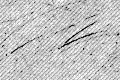
\includegraphics[width=.4\textwidth]{05_ergebnisse/ergDiskussion/figures/polierfehler}};
	\node [below=0.2cm of img2] {Ausschnitt von Brillenglas 2};
	
\end{tikzpicture}
\caption[Erkennbare kleine Defekte oder Laser-Gravur]{Erkennbare kleine Defekte oder Laser-Gravuren durch Durchlichtauswertung mit Verfahren \glqq Sichtprüfung durch Lichtstreuung\grqq ~(siehe Kapitel \ref{chp:sichtpruefungDurchLichtstreuung}) Linkes Teilbild: Erkennbare Lasergravur, Rechtes Teilbild: Leichte Kratzer durch Fehler bei der Polierung}
		\label{tikz:abbErkennbareKleineDefekteLichtstreuung}
	\end{figure}
}

\noindent
Außerdem ist es möglich für transparente Objekte durch die Durchlichtauswertung auch Defekte im Objekt, wie z. B. Lufteinschlüsse in Gläsern festzustellen.
Dies konnte allerdings nicht nachgeprüft werden, da solche Defekte in den zur Verfügung stehenden Prüfobjekten nicht vorhanden waren.

\p
Für nicht-transparente Prüfobjekte kann das Verfahren \glqq Sichtprüfung durch Lichtstreuung\grqq ~durch eine Spiegelbildaufwertung ebenfalls verwertbare Bilder erzeugen um Defekte zu detektieren, allerdings gibt es hierbei schon erste Probleme.
Eine große Schwäche des Verfahrens ist die Abhängigkeit von Oberflächenbeschriftungen oder -aufdrucken.
Da stets Grauwerte der Kamerabilder verknüpft werden beeinflussen unterschiedliche Farben auf der Oberfläche das Ergebnis (siehe Abbildung \ref{img:delleBeschriftung}).
Das gleiche Phänomen lässt sich auch beobachten wenn das Objekt abhängig von der Position unterschiedlich stark reflektierend ist.

% Abbildung: Beschriftung Delle
{
	\begin{figure}[H]
		\centering
		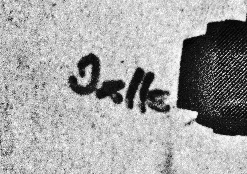
\includegraphics[width=0.4\textwidth]{05_ergebnisse/ergDiskussion/figures/delleBeschriftung}
		\caption[Sichtbare Beschriftung nach Anwendung des Verfahrens aus Kapitel \ref{chp:sichtpruefungDurchLichtstreuung}]{Sichtbare Beschriftung \glqq Delle\grqq ~nach Anwendung des Verfahren \glqq Sichtprüfung durch Lichtstreuung\grqq auf Keramikobjekt 2. Ausschnitt aus Abbildung \ref{tikz:abbNachbearbeitungSpLichtstreuung}}
		\label{img:delleBeschriftung}
	\end{figure}
}

\noindent
Dieser Einfluss kann zu Problemen in der nachfolgenden Auswertung des Ergebnisbilds durch herkömmliche Bildverarbeitungsalgorithmen führen.
Für dieses Verfahren ist es also notwendig, dass das Prüfobjekt einfarbig und ohne Beschriftungen vorliegt.
Außerdem sollte das Prüfobjekt an allen zu untersuchenden Stellen das Licht gleich stark reflektieren.
Damit können kleinere Defekte, wie z. B. Oberflächenpickel oder Kratzer in Brillengläsern detektiert werden.
Größere Defekte wie z. B. die Delle auf der Oberfläche des Keramikobjekts 2 (siehe Abbildung \ref{tikz:abbNachbearbeitungSpLichtstreuung}) sind hingegen schwerer zu identifizieren.
Dieselben Effekte in den Ergebnisbildern wie bei Dellen können auch bei stärker gekrümmten Objekten oder an matten Stellen auftreten.

\p
Die deflektometrische Registrierung erzeugt lediglich Zuordnungsinformationen die durch spezielle Algorithmen weiterverarbeitet werden muss um Untersuchungen der Oberfläche zu treffen.
In dem Abschnitt \ref{sec:ergebnisseDeflektometrischeRegistrierung} wurde zunächst ein Bild aus der  deflektometrischen Registrierung der Zeilen erzeugt, dass man Bildverarbeitungsalgorithmen anwenden kann um bestimmte Auffälligkeiten hervorheben zu können.
Allerdings verliert man nach dem vorgestellten Ansatz eventuell Informationen über sehr kleine Defekte, da bei der Bilderzeugung je nach verwendeter Farbtiefe mehrere Zeilenpositionen demselben Grauwert zugeordnet werden.
Man verliert kleine Details der deflektometrischen Registrierung, das macht es schwieriger sehr kleine Abweichungen der Reflexionen, wie z. B. Kratzer oder Laser-Gravuren zu erkennen.
Die tatsächlichen Reflexionsabweichungen sind bei der Durchlichtauswertung kleiner als bei dem Spiegelbild.
Es lässt sich auch in Abbildung \ref{tikz:abbAbleitungRegistrierungDurchlicht} erkennen, dass sich das Verfahren für die Durchlichtauswertung von Brillengläsern nur begrenzt eignet.
Auch die Auswertung des Spiegelbilds von Brillenglas 1 zeigt keine Auffälligkeiten, da die Kratzer und Laser-Gravuren die Reflexion des Lichts nur minimal beeinflussen (siehe Abbildung \ref{tikz:abbAbleitungRegistrierungSpiegel}).

\p
Für die Spiegelbildauswertung durch Bestimmung der deflektometrischen Registrierung der Zeilen sind für die untersuchten Keramikobjekte bessere Ergebnisse zu erkennen (siehe Abbildung \ref{tikz:abbErkennbareDefekteRegistrierung}).

% Abbildung: Erkennbare Defekte
{
	\begin{figure}[H]
		\centering
		\begin{tikzpicture}[every node/.style={inner sep=0,outer sep=0}]

	\node [anchor=north east] (img1) at (-0.03\textwidth,0) {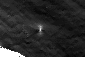
\includegraphics[width=.4\textwidth]{05_ergebnisse/ergDiskussion/figures/pickel}};
	\node [below=0.2cm of img1, align=center] {Ausschnitt von Keramikobjekt 1 \\ aus Abbildung \ref{tikz:abbAbleitungRegistrierungSpiegel}};
	\node [anchor=north west] (img2) at (0.03\textwidth,0) {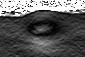
\includegraphics[width=.4\textwidth]{05_ergebnisse/ergDiskussion/figures/delle}};
	\node [below=0.2cm of img2, align=center] {Ausschnitt von Keramikobjekt 2 \\ aus Abbildung \ref{tikz:abbAbleitungRegistrierungSpiegel}};
	
\end{tikzpicture}
\caption[Erkennbare Oberflächendefekte durch deflektometrische Registrierung]{Erkennbare Oberflächendefekte durch Ableitung der deflektometrischen Registrierung. Linkes Teilbild: Oberflächenpickel, Rechtes Teilbild: Delle in der Oberfläche}
		\label{tikz:abbErkennbareDefekteRegistrierung}
	\end{figure}
}

\noindent
%TODO MACH DIE SCHEISSE FERTIG!!!
%TODO Pro: Oberflächenbeschriftungen/-aufdrucke
%TODO Pro: tatsächliche Krümmungsinformationen vorhanden
%TODO Contra: Fremdlicheinwirkungen und ungewollte Reflexionen -> Übergang zu Rückseitenreflex
%TODO Rückseitenreflex -> Zeige Beispielbild von deflektometrische Registrierung -> Übergang zu Rückseitenreflex bei Sichtprüfung mit Lichtstreuung
%TODO Konkreter Vergleich der Ergebnisse (Ansprechen von Stabilität des Lichtstreuungsverfahren und Weiterverarbeitbarkeit)-> Empfehlungen des Verfahrens für die jeweilige Anwendung (mit Aufbauempfehlung)
%TODO Aber: Laufzeit entscheidend für die Anwendung -> Zeige Laufzeitdiagramme
%TODO Abschluss :D